\section{The Space of Pentatonic Scales}
El sistema tonal que solem utilitzar consta de 12 semitons Do-Do\#-Re-Re\#-Mi... Cada to només té lloc una vegada a cada octava. Una bona manera de veure aquesta col·lecció de tons és col·locar-los formant un cercle i oblidant-nos de la informació sobre l'octava.  La imatge de l'esquerra mostra les dotze notes en la seva distribució habitual de tecles blanques i negres d'un piano. Els cercles blancs formen la més que coneguda escala de Do major. Però tocar només les notes de les tecles negres també sona interessant. Formen el que s'anomena una escala pentatònica: una col·lecció de cinc notes en una octava. Formar melodies amb aquestes notes recorda a música d'orient. Si rotem el patró cíclicament, creem fins a 12 escales pentatòniques.


\begin{figure}[h]
\centering
\begin{subfigure}{0.45\textwidth}
\centering
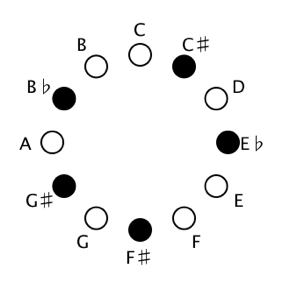
\includegraphics[width=0.9\textwidth]{PentatonicScales_1}
\end{subfigure}
\begin{subfigure}{0.45\textwidth}
\centering
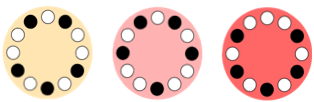
\includegraphics[width=\textwidth]{PentatonicScales_2}
\end{subfigure}
\end{figure}

Hi ha un munt d'altres maneres de seleccionar 5 notes de les 12 del nostre sistema tonal. De totes maneres, si volem fer distribucions de forma més o menys igual, també podem requerir que no se seleccionin notes ``veïnes''. Amb aquestes condicions trobem dues maneres més de distribuir les cinc notes. Cada una d'aquestes maneres pot trobar-se en 12 rotacions diferents (fes una ullada a la imatge).

\paragraph{La Música:} Les escales pentatòniques tenen una mena de so lliure que no recorden ni a un mode major ni menor. Algunes aporten molta pau (la groga) i d'altres tenen molta tensió. Aquestes escales s'han utilitzat pels compositors de l'època impressionista com Debussy. Altres creen sons molt alegres que recorden a imatges d'altres cultures. Debussy, per exemple, es va interessar en les escales pentatòniques després de sentir la música dels gamelan de Java i Bali.

\paragraph{Les Mates:}  La imatge mostra l'espai de totes les pentatòniques anteriorment. Cada un dels tipus té lloc en 12 posicions rotacionals. A la imatge les escales estan ordenades de manera que dos dels tipus es connecten amb un arc si només es diferencien per exactament un semitò. Pots veure ``l'espai d'escales pentatòniques''

\paragraph{El Mòdul:} Al mòdul, pots triar reproduir una peça d'un compositor clàssic (Mozart, Bach, Debussy, Liszt i altres), però aquesta peça no sonarà exactament com diu a la partitura. També pots triar una escala pentatònica i cada nota de la peça es canviarà per la nota més propera dins de l'escala que has triat. També pots canviar l'escala mentre la música va sonant. D'aquesta manera pots crear la teva pròpia música impressionista.

\begin{figure}
\centering
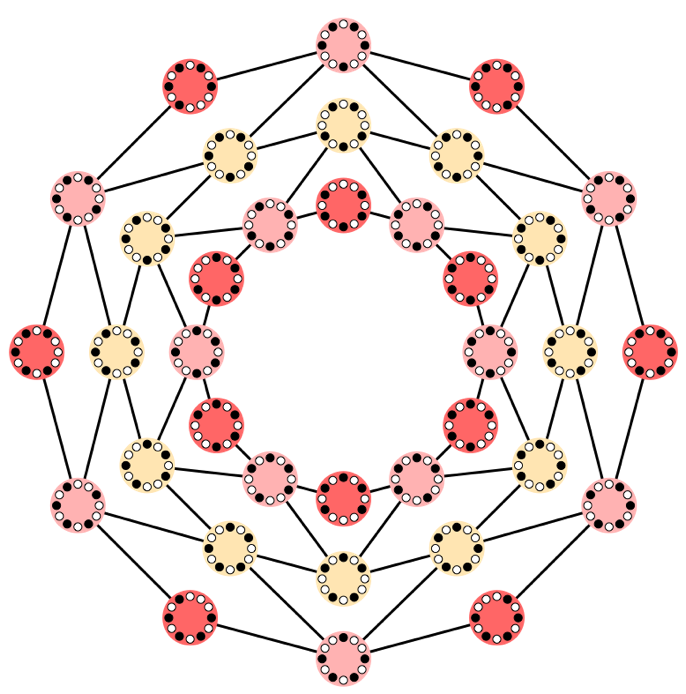
\includegraphics[width=0.6\textwidth]{PentatonicScales_3}
\end{figure}

\vfill

Autor del mòdul: Jürgen Richter-Gebert, Technical University of Munich
Motor de so: Patrick Wilson i Aaron Montag / basat en CindyJS.org.
Música: Bach. Preludi i Fuga en Do Major BWV 846 / Mozart, Sonata No. 16 en Do Major (Sonata facile), KV 545 / Liszt, Hungarian Rhapsody No 9 / Chopin, Preludi No 4  en Mi menor. Gravat per Bernd Krueger, Alemanya / Gershwin. Rhapsody in Blue / Debussy, Arabesque 1 / Debussy, Images -- Reflets dans l'eau. Tocat per Katsuhiro Oguri, Japó.
